\begin{frame}[fragile]{Visualização de um grafo conectado e caminhos}

    \begin{figure}
        \centering

        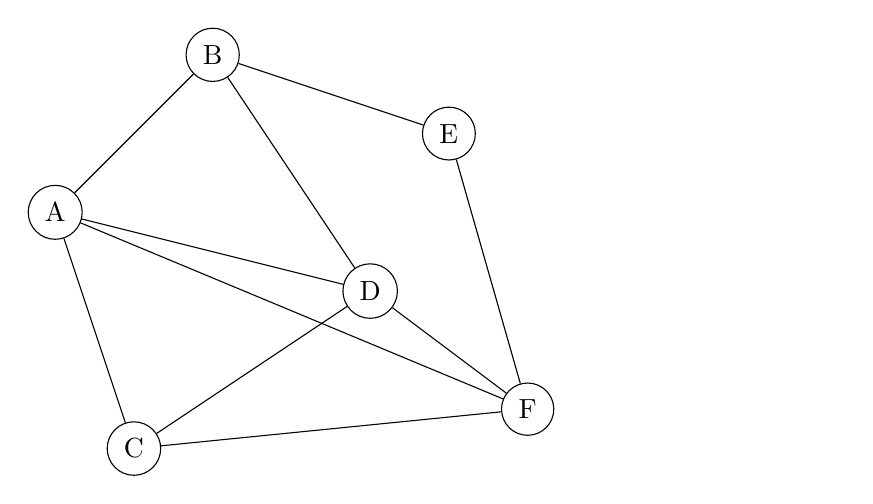
\begin{tikzpicture}
            \node[draw,circle] (A) at (0, 3) { A };
            \node[draw,circle] (B) at (2, 5) { B };
            \node[draw,circle] (C) at (1, 0) { C };
            \node[draw,circle] (D) at (4, 2) { D };
            \node[draw,circle] (E) at (5, 4) { E };
            \node[draw,circle] (F) at (6, 0.5) { F };

            \draw (A) to (B);
            \draw (A) to (C);
            \draw (D) to (C);
            \draw (E) to (B);
            \draw (A) -- (D);
            \draw (A) -- (F);
            \draw (B) -- (D);
            \draw (C) to (F);
            \draw (D) -- (F);
            \draw (E) -- (F);

            \draw[opacity=0,blue] (7, 5) -- (7.5, 5) node[anchor=west,black] { \scriptsize Caminho de A a F };

        \end{tikzpicture}

    \end{figure}

\end{frame}

\begin{frame}[fragile]{Visualização de um grafo conectado e caminhos}

    \begin{figure}
        \centering

        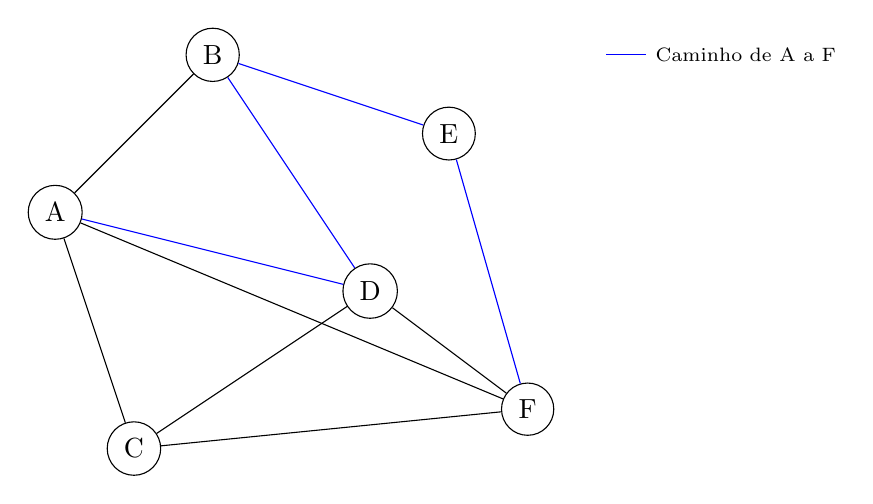
\begin{tikzpicture}
            \node[draw,circle] (A) at (0, 3) { A };
            \node[draw,circle] (B) at (2, 5) { B };
            \node[draw,circle] (C) at (1, 0) { C };
            \node[draw,circle] (D) at (4, 2) { D };
            \node[draw,circle] (E) at (5, 4) { E };
            \node[draw,circle] (F) at (6, 0.5) { F };

            \draw (A) to (B);
            \draw (A) to (C);
            \draw (D) to (C);
            \draw[blue] (E) to (B);
            \draw[blue] (A) -- (D);
            \draw (A) -- (F);
            \draw[blue] (B) -- (D);
            \draw (C) to (F);
            \draw (D) -- (F);
            \draw[blue] (E) -- (F);

            \draw[blue] (7, 5) -- (7.5, 5) node[anchor=west,black] { \scriptsize Caminho de A a F };

        \end{tikzpicture}

    \end{figure}

\end{frame}

\begin{frame}[fragile]{Visualização de um grafo conectado e caminhos}

    \begin{figure}
        \centering

        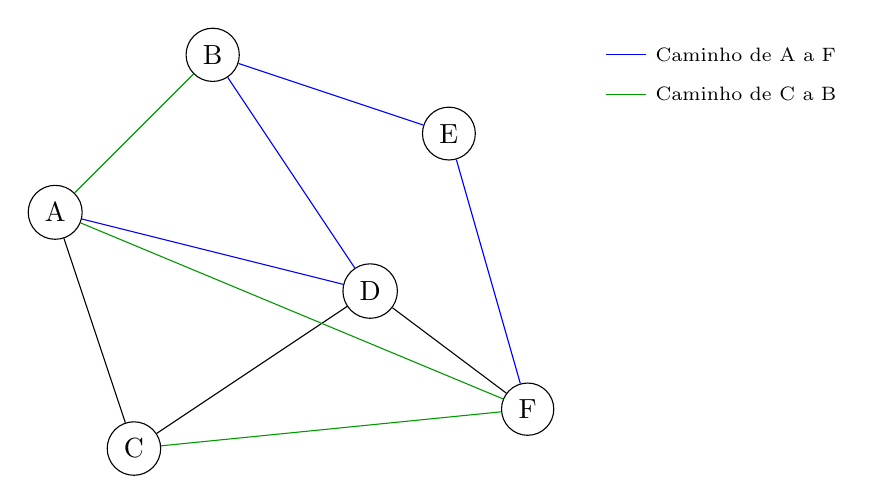
\begin{tikzpicture}
            \node[draw,circle] (A) at (0, 3) { A };
            \node[draw,circle] (B) at (2, 5) { B };
            \node[draw,circle] (C) at (1, 0) { C };
            \node[draw,circle] (D) at (4, 2) { D };
            \node[draw,circle] (E) at (5, 4) { E };
            \node[draw,circle] (F) at (6, 0.5) { F };

            \draw[green!60!black] (A) to (B);
            \draw (A) to (C);
            \draw (D) to (C);
            \draw[blue] (E) to (B);
            \draw[blue] (A) -- (D);
            \draw [green!60!black](A) -- (F);
            \draw[blue] (B) -- (D);
            \draw[green!60!black] (C) to (F);
            \draw (D) -- (F);
            \draw[blue] (E) -- (F);

            \draw[blue] (7, 5) -- (7.5, 5) node[anchor=west,black] { \scriptsize Caminho de A a F };
            \draw[green!60!black] (7, 4.5) -- (7.5, 4.5) node[anchor=west,black] { \scriptsize Caminho de C a B };

        \end{tikzpicture}

    \end{figure}

\end{frame}

\begin{frame}[fragile]{Visualização de um grafo conectado e caminhos}

    \begin{figure}
        \centering

        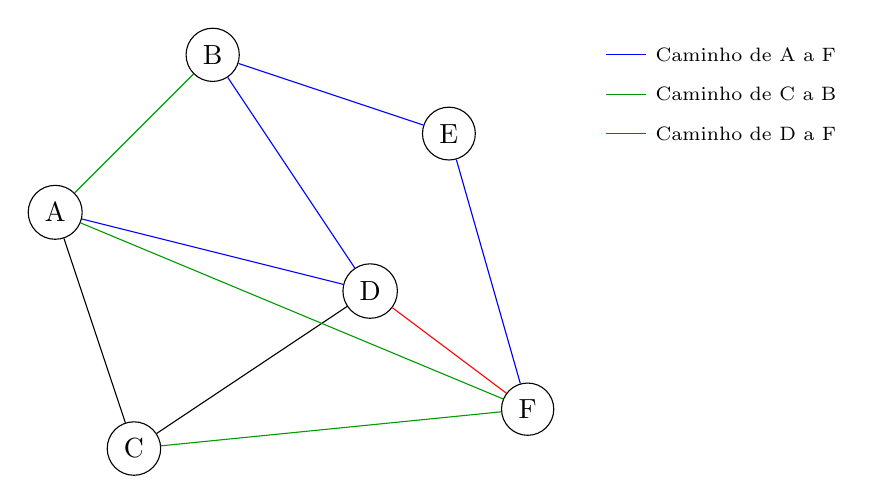
\begin{tikzpicture}
            \node[draw,circle] (A) at (0, 3) { A };
            \node[draw,circle] (B) at (2, 5) { B };
            \node[draw,circle] (C) at (1, 0) { C };
            \node[draw,circle] (D) at (4, 2) { D };
            \node[draw,circle] (E) at (5, 4) { E };
            \node[draw,circle] (F) at (6, 0.5) { F };

            \draw[green!60!black] (A) to (B);
            \draw (A) to (C);
            \draw (D) to (C);
            \draw[blue] (E) to (B);
            \draw[blue] (A) -- (D);
            \draw [green!60!black](A) -- (F);
            \draw[blue] (B) -- (D);
            \draw[green!60!black] (C) to (F);
            \draw[red] (D) -- (F);
            \draw[blue] (E) -- (F);

            \draw[blue] (7, 5) -- (7.5, 5) node[anchor=west,black] { \scriptsize Caminho de A a F };
            \draw[green!60!black] (7, 4.5) -- (7.5, 4.5) node[anchor=west,black] { \scriptsize Caminho de C a B };
            \draw[red] (7, 4) -- (7.5, 4) node[anchor=west,black] { \scriptsize Caminho de D a F };

        \end{tikzpicture}

    \end{figure}

\end{frame}

